%!TEX root=../protocol.tex	% Optional

\section{Lösung}

\subsection{Projekt migrieren}

Da die Aufgabe die bestehende Aufgabe \textbf{'Message Oriented Middleware'} erweitert, wird die gesamte Codebase als Grundlage weiterverwendet.

Das Projekt bestand aus einem Windpark welcher eine Liste aus Windrädern besitzt.

Außerdem gibt es eine Zentrale welche über die Middleware die Informationen des Windparks erhält.

Dies soll erweitert werden, sodass statt der \textbf{Message Oriented} Middleware eine \textbf{Document Oriented} Middleware verwendet wird.

\clearpage
\subsubsection{Neues Projekt erstellen}

Das erstellen des neuen Projektes erfolgt mit dem \textbf{Spring Initializr}.

Folgende allgemeine Projekt Einstellungen habe ich konfiguriert:

\begin{figure}
    \caption{Spring Initializr Projektkonfiguration}
    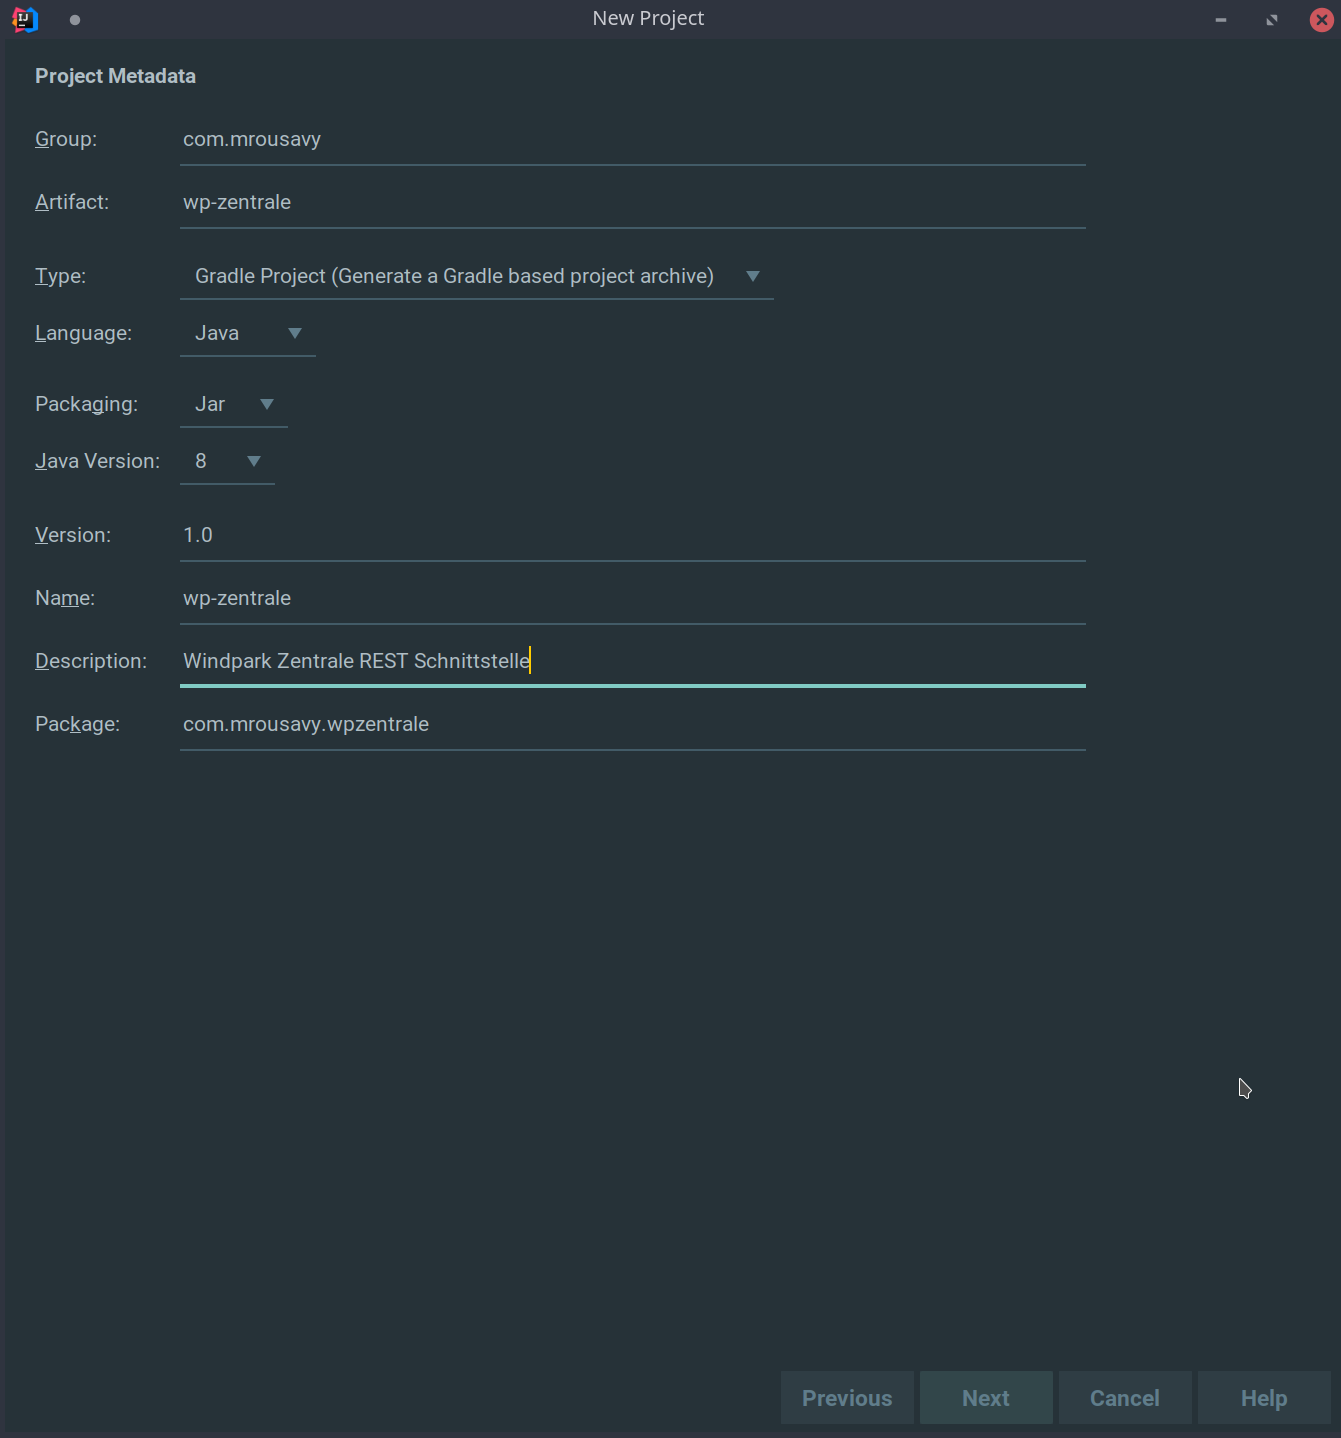
\includegraphics[width=15cm]{images/initializr-general}
    \centering
\end{figure}

Sowie folgende Frameworks für das Windpark Projekt:

\begin{figure}
    \caption{Spring Initializr Framework Konfiguration}
    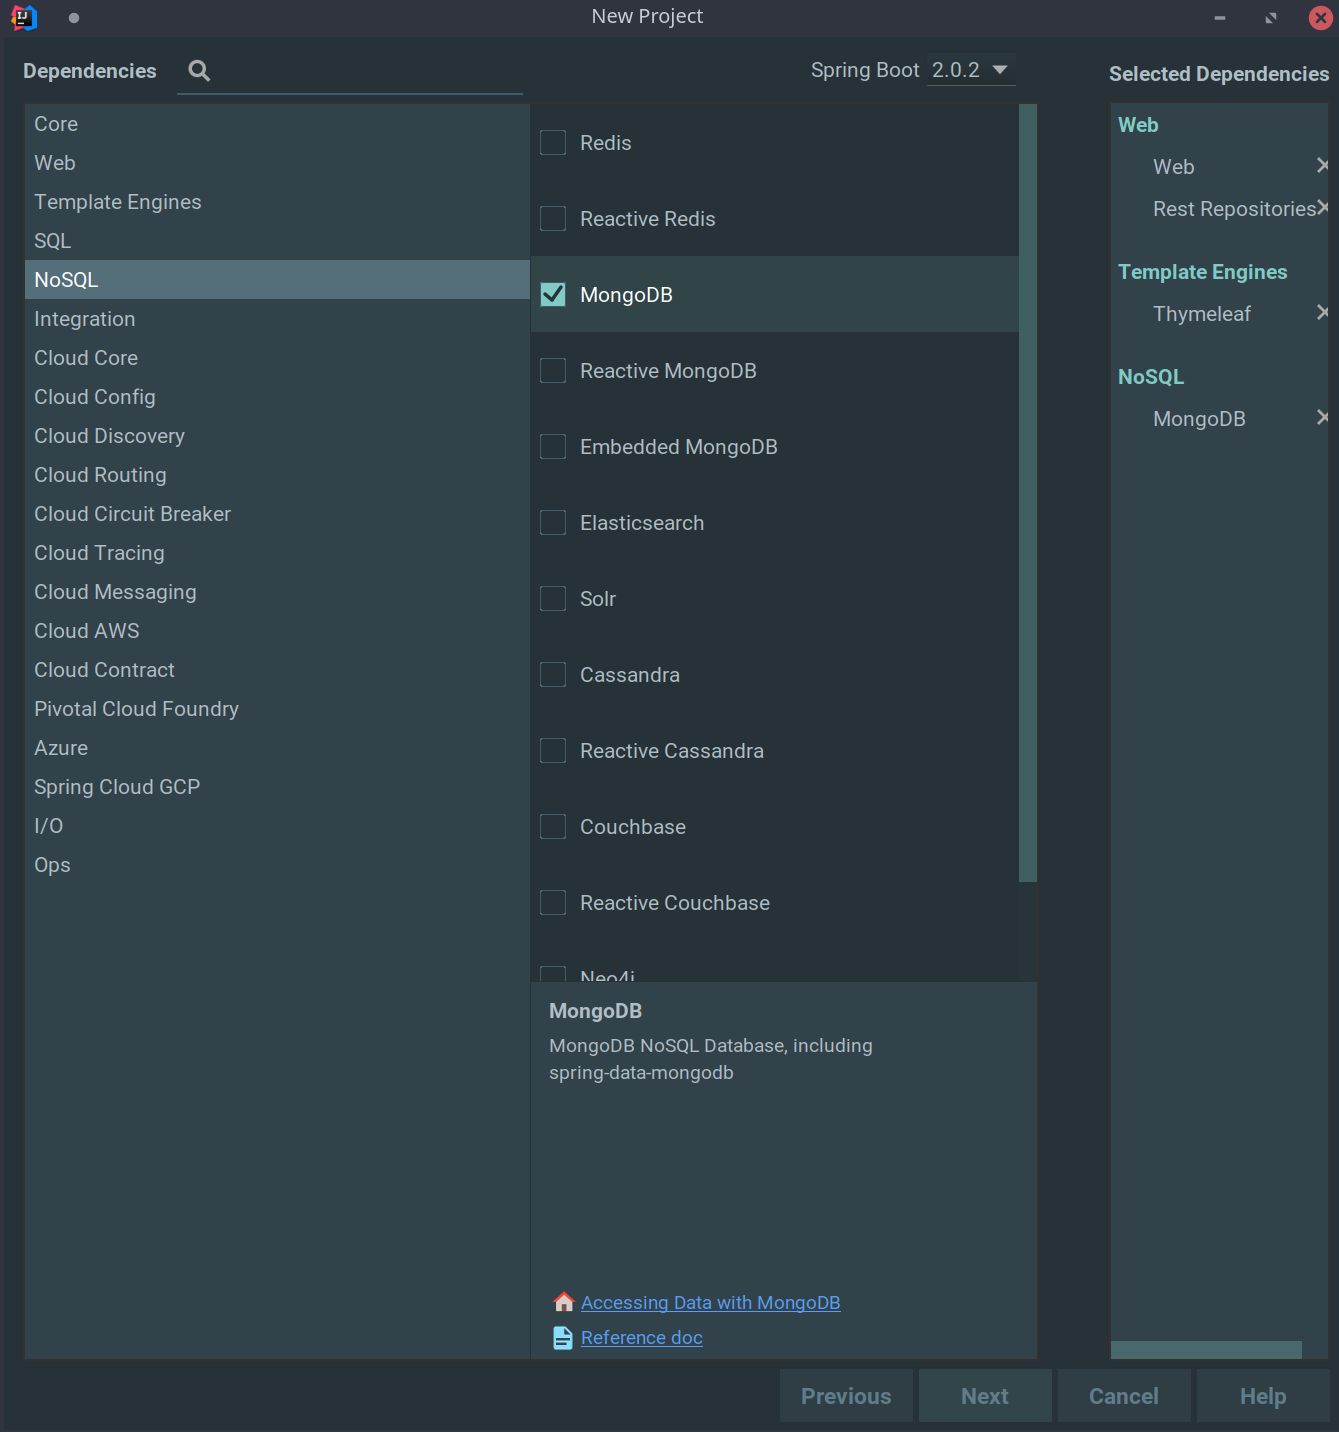
\includegraphics[width=15cm]{images/initializr-frameworks}
    \centering
\end{figure}

\clearpage
\subsection{Windpark}

\subsubsection{Allgemein}

Eine Spring Web Application wird nun einen einzelnen Windpark darstellen.

Es wird also zusätzlich zu folgender Application Klasse:

\begin{code}{java}
    package com.mrousavy.wpwindpark;

    import org.springframework.boot.SpringApplication;
    import org.springframework.boot.autoconfigure.SpringBootApplication;

    @SpringBootApplication
    public class WpWindparkApplication {
        public static void main(String[] args) {
            SpringApplication.run(WpWindparkApplication.class, args);
        }
    }
\end{code}

.., welche mittels des \textit{Spring Initializr} automatisch erstellt wurde, noch ein \textbf{ReST Controller} erstellt.

\subsubsection{ReST Controller}

Dieser \textbf{ReST Controller} kümmert sich um alle Anfragen über \textit{HTTP/HTTPS}, und liefert einen \texttt{String} zurück.

Definiert werden \textbf{ReST Controller} in \textbf{Spring} mittels der \texttt{@RestController} Annotation:

\begin{code}{java}
    @RestController
    public class WindparkRestController {
\end{code}

Sobald also die Spring Application über die URL beispielsweise in einem Browser aufgerufen wird, sucht \textbf{Spring} einen passenden \textbf{ReST Controller} um die Anfrage zu verarbeiten. Dies gelangt zur Laufzeit mittels der vorhin erwähnten \texttt{@RestController} Annotation.

Wir können einerseits einen \textit{Index} (also die Startseite, beispielsweise erreichbar unter \texttt{172.0.1.2}), oder eine Subseite (beispielsweise erreichbar unter \texttt{172.0.1.2/hello}) definieren. Hierbei verwenden wir die Spring Web Annotation \texttt{@GetMapping(String)}.

Um einen Wert (\texttt{String}) zurückzugeben, wird die Spring Web Annotation {\texttt{@ResponseBody}} verwendet.

Also können wir beispielsweise folgende Funktion definieren:

\begin{code}{java}
    @GetMapping("/hello")
    @ResponseBody
    public String sayHello() {
        return "<p>Hello world!</p>";
    }
\end{code}

Der Windpark Controller ist so aufgebaut, dass damit gerechnet wird, dass ein vorgefertigtes \texttt{XML} File auf dem Server abgespeichert ist, welches über eine \textit{ReST GET-Function} abgerufen wird.

Um eine Text-Datei in Java 7 zu lesen, wird der \texttt{BufferedReader} verwendet. Es wird mit der \texttt{BufferedReader.getLine()} Methode gearbeitet.

\begin{code}{java}
    package com.mrousavy.wpwindpark;

    import org.springframework.web.bind.annotation.GetMapping;
    import org.springframework.web.bind.annotation.ResponseBody;
    import org.springframework.web.bind.annotation.RestController;

    @RestController
    public class WindparkRestController {

        private final String FILE_NAME = "parknodedata.xml";

        public String readXml() throws IOException {
            try (BufferedReader br = new BufferedReader(new FileReader(FILE_NAME))) {
                StringBuilder builder = new StringBuilder();

                String sCurrentLine;
                while ((sCurrentLine = br.readLine()) != null) {
                    builder.append(sCurrentLine);
                }

                return builder.toString();
            }
        }
    }
\end{code}

\subsubsection{JSON}

Außerdem wird die Dependency \texttt{org.JSON} verwendet, um das XML zu einem JSON Format zu konvertieren:

\begin{code}{properties}
    dependencies {
        compile('org.springframework.boot:spring-boot-starter-data-rest')
        compile('org.springframework.boot:spring-boot-starter-web')
        compile('org.jdom:jdom2:2.0.6')
        compile('xerces:xercesImpl:2.11.0')
        compile group: 'org.json', name: 'json', version: '20180130'
        testCompile('org.springframework.boot:spring-boot-starter-test')
    }
\end{code}

Der vollständige Code des \textbf{ReST Controllers} sieht nun folgendermaßen aus:

\begin{code}{java}
    @RestController
    public class WindparkRestController {

        private final String FILE_NAME = "parknodedata.xml";

        public String readXml() throws IOException {
            try (BufferedReader br = new BufferedReader(new FileReader(FILE_NAME))) {
                StringBuilder builder = new StringBuilder();

                String sCurrentLine;
                while ((sCurrentLine = br.readLine()) != null) {
                    builder.append(sCurrentLine);
                }

                return builder.toString();
            }
        }

        @GetMapping("/xml")
        @ResponseBody
        public String getXml() {
            System.out.println("Working Directory = " + System.getProperty("user.dir"));

            try {
                return readXml();
            } catch (Exception e) {
                e.printStackTrace();
                return "<error>" + e.getMessage() + "</error>";
            }
        }


        @GetMapping("/json")
        @ResponseBody
        public String getJson() {
            System.out.println("Working Directory = " + System.getProperty("user.dir"));

            try {
                String xml = readXml();

                JSONObject json = XML.toJSONObject(xml);
                String prettyJson = json.toString(4);
                System.out.println("Read JSON: " + prettyJson);
                return prettyJson;
            } catch (Exception e) {
                e.printStackTrace();
                return "<error>" + e.getMessage() + "</error>";
            }
        }
    }
\end{code}

\subsubsection{Port}

Da wir mehrere Windparks auf einem Host starten möchten, müssen wir Spring mitteilen, verschiedene Ports für den Tomcat Server zu verwenden.

Hierzu verwenden wir die \texttt{application.properties} Datei:

\begin{code}{properties}
    server.port = 8081
\end{code}


\subsubsection{Start}

Sobald wir die Main-Methode starten, wird der Spring Server initialisiert:

\begin{figure}
    \caption{Spring Console Output - Initialization}
    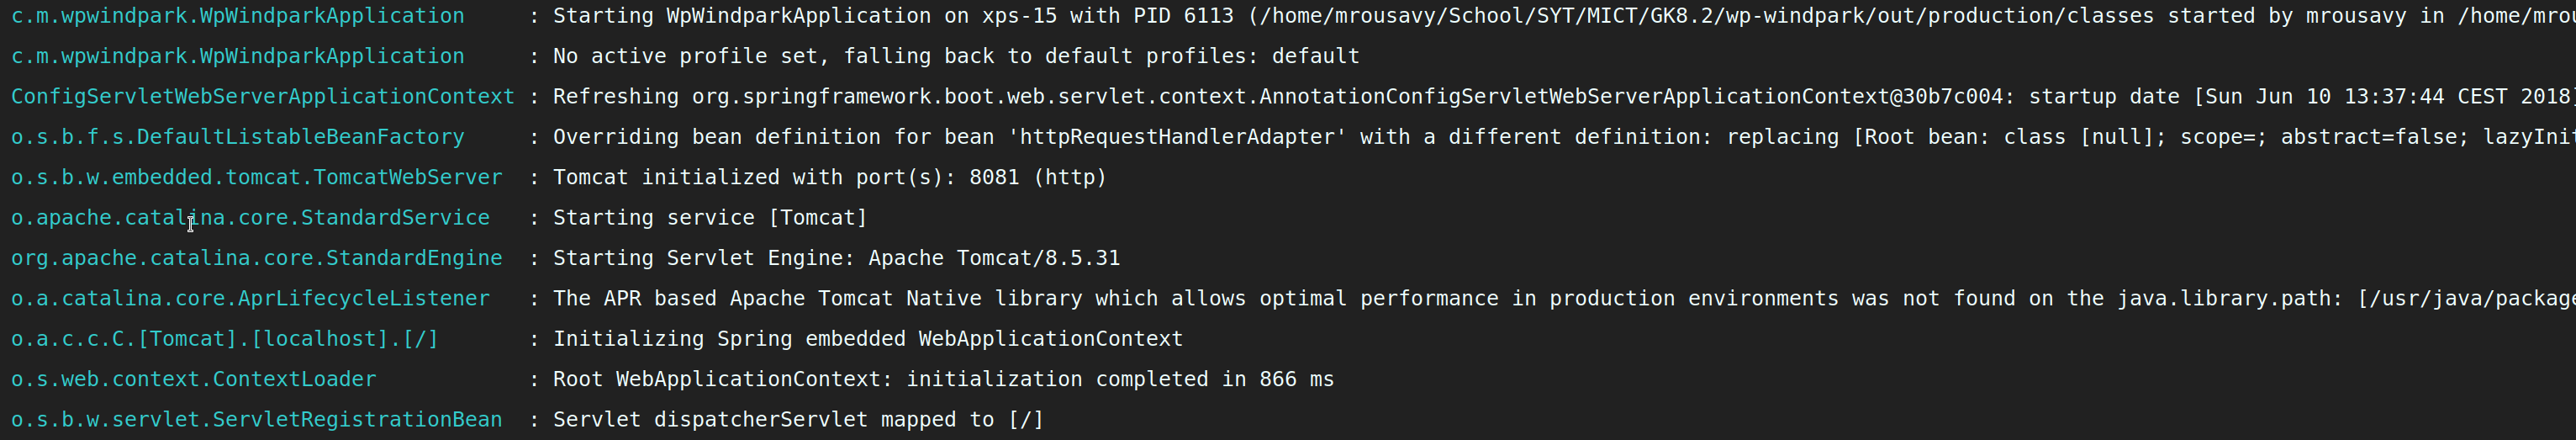
\includegraphics[width=15cm]{images/spring-console-init}
    \centering
\end{figure}

Außerdem wird hier die \texttt{/xml} \textbf{ReST Schnittstelle} "gemapped":

\begin{figure}
    \caption{Spring Console Output - XML ReST Interface Mapping}
    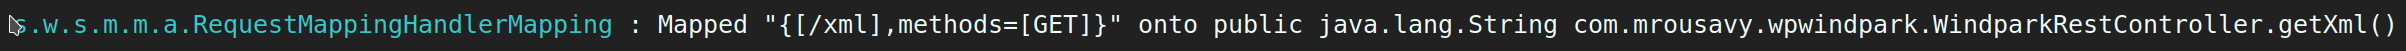
\includegraphics[width=15cm]{images/spring-console-mapped}
    \centering
\end{figure}

Zuletzt wird der Tomcat Server gestartet:

\begin{figure}
    \caption{Spring Console Output - Tomcat Server Start finish}
    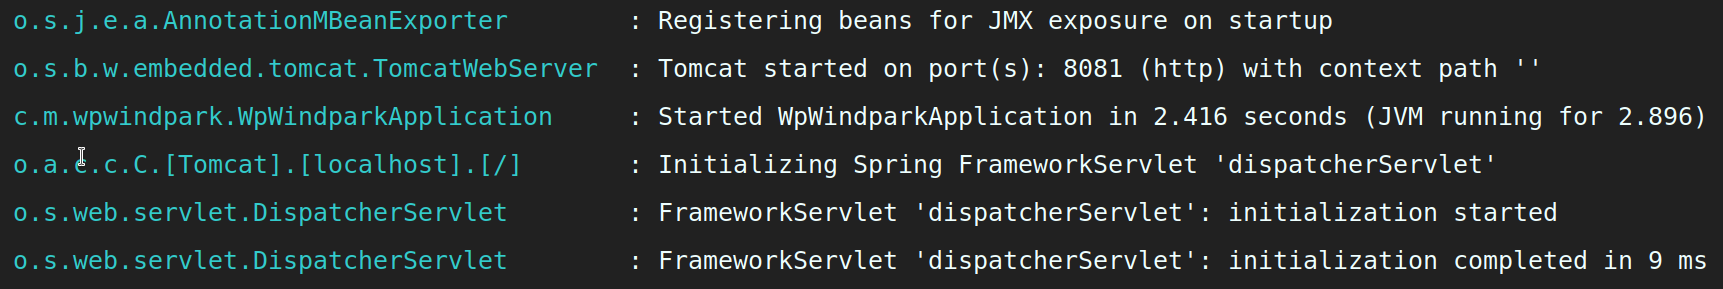
\includegraphics[width=15cm]{images/spring-console-finish}
    \centering
\end{figure}

Die Spring Application ist nun erreichbar unter \texttt{localhost:8081/xml}.

\begin{figure}
    \caption{Spring Application Web-Aufruf (JSON)}
    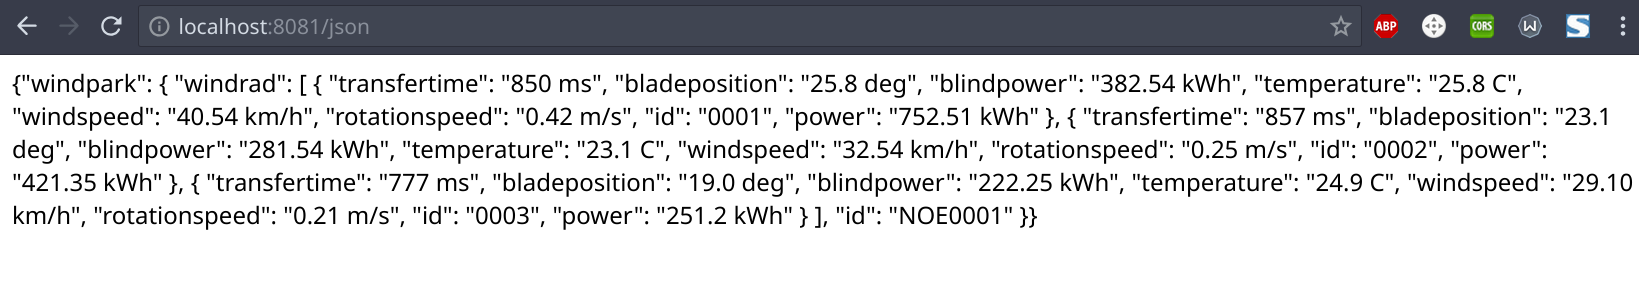
\includegraphics[width=15cm]{images/spring-app-json}
    \centering
\end{figure}

Und falls es irgendeinen Fehler in der Applikation gibt:

\begin{figure}
    \caption{Spring Application Web-Aufruf - Error caught}
    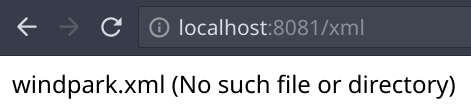
\includegraphics[width=15cm]{images/spring-app-filenotfound}
    \centering
\end{figure}


\clearpage
\subsection{Zentrale}

\subsubsection{Allgemein}

Nun erstellen wir eine \textbf{Spring Application} welche eine \textbf{Windpark Zentrale} repräsentiert.

Der Aufbau dieser \textbf{Spring Application} ist folgendermaßen gedacht:

\begin{itemize}
    \item Es werden mehrere Windparks eingetragen welche überwacht werden sollen. Diese Windparks werden mittels ihrer \textbf{ReST} Addresse eingetragen (also \textbf{IP}, \textbf{Port} und \textbf{Subseite} - beispielsweise: \texttt{172.0.1.2:8081/xml})
    \item Diese einzelnen Windparks werden über Ihre \textbf{ReST} Schnittstelle \textit{durch-iteriert}, und einzeln \textit{geparsed}.
    \item Nun werden die Windparks mittels Aufzeichnungsdatum fortlaufend auf einer \textbf{NoSQL MongoDB Datenbank} im \textbf{JSON} Format abgespeichert.
    \item Verwaltet werden diese Daten mittels den \textbf{MongoDB} Tools (Mongo Shell)
    \item Zusätzlich soll ein Webinterface erstellt werden, wo die Daten von der Mongo Datenbank angezeigt werden.
\end{itemize}

\subsubsection{Model}

Es wird ein \textbf{Model} definiert, welches die einzelnen Windräder, Windparks und Windpark Versionen als POJOs (\textbf{P}lain \textbf{O}ld \textbf{J}ava \textbf{O}bjects) repräsentiert.

Also werden die Klassen \texttt{Windpark.java}, \texttt{Windrad.java} und \texttt{WindparkVersion.java} erstellt, welche für den \textbf{MongoDB} Zugriff auch noch Mongo Repositories benötigen.

Ein Mongo Repository verwaltet die Schnittstelle zwischen der Java Runtime und dem MongoDB Treiber. Für den Java Code ist es also quasi die Schnittstelle zur Datenbank.

Eine Repository könnte beispielsweise folgendermaßen aussehen:

\begin{code}{java}
    public interface WindparkRepository extends MongoRepository<Windpark, String> {
        public Windpark findByid(String id);
    }
\end{code}

\subsubsection{Data Access Layer}

Um die einzelnen Daten nun von den Windparks zu bekommen, erstellen wir einen \textbf{Data Access Layer}, welcher folgende Aufgaben hat:

\begin{itemize}
    \item Windpark Zentrale Config lesen (zu überwachende Windparks auslesen)
    \item Windparks JSON auslesen über deren ReST Schnittstelle
    \item Einzelne Windparks Zusammenfassen
    \item Auf MongoDB Datenbank fortlaufend speichern
\end{itemize}






\clearpage
\section{Fragen}

\begin{itemize}
    \item Nennen Sie 5 Vorteile eines NoSQL Repository im Gegensatz zu einem relationalen DBMS
    \item Nennen Sie 4 Nachteile eines NoSQL Repository im Gegensatz zu einem relationalen DBMS
    \item Welche Schwierigkeiten ergeben sich bei der Zusammenführung der Daten?
    \item Können die Daten der MongoDB von Mitarbeitern geändert werden?
        Ja/Nein, Begründen Sie Ihre Antwort.
    \item Beschreiben Sie die wichtigsten Eigenschaften des Spring Frameworks?
    \item Was versteht man unter dem Spring Boot Projekt?
    \item Nennen Sie jeweils 3 Argumente für und gegen den Einsatz von Spring bei der Entwicklung solcher Projekte
\end{itemize}
